\chapter*{Blog}
        \addcontentsline{toc}{chapter}{Blog}
        \chaptermark{Blog}
	\markboth{Blog}{Blog}
	
	This is the portion of the thesis that I will update regularly with rough notes, lit reviews, results, etc. some of which will be worked in to the real document after some polishing. 
	\section{Goals}
	\begin{itemize}
	\item{10/14: Define specific problem.}
	\item{Fall Break: Experimental Setup}
	\item{Winter Break: Lit Review Complete}

	\end{itemize}

	
	
	\section{To Do}
	\begin{itemize}
	\item{Obtain flashdrives.    Miguel 9/30/14}
	\item{Set up digital camera.    Miguel 9/30/14}
	\item{Double Sided Tape.    Miguel 10/7/14}
	\item{Accelerometer.    Miguel 10/7/14}
	\item{Tray geometry for aiming droplets.    Miguel 10/7/14}
	\end{itemize}
	
	\subsection{Done}
	\begin{itemize}
	\item{Learn how to use the new \LaTeX\ and Github setup.     Miguel 9/30/14}
	\end{itemize}
	
	\section{Literature Reviews}
	
	    \subsection{Particle-wave association on a fluid interface (Protiere 2006)}
	
	    \subsection{Pilot-Wave Hydrodynamics (Bush 2015)}
	    In this annual review, Bush describes some of the characteristics of the bouncing oil drop experiment that are analagous to effects witnessed in the quantum mechanical world (single-particle diffraction, tunneling, quantized orbits, orbital level splitting, and spin states). Dynamics of the walker are described mathematically. Finally, comparisons to de Broglie's orginal formulation of QM (and not Bohm's) and Stochastic Electrodynamics (?) are made. 
	    \subsubsection{Basic Parameters}
	       Consider a fluid of density $\rho$, viscosity $\nu$, and surface tension $\sigma$, in a bath of depth $H$ driven vertically at an amplitude $A_0$ at frequency $f=\omega/{2\pi}$. By defining $\mathnormal{\gamma}=A_0\omega^2$, the effective gravity in the frame of reference of the bath is $g+\gamma~\mathrm{sin}(\omega t)$. The oil droplet of diameter $D$ bounces in the regime $\gamma<\gamma_F$, where $\gamma_F$ is the Faraday threshold (at this point, Fraday waves appear). The important experimental limits are outlined in \refTab{approxlimits}. 
	       \begin{table}[htdp] 
\caption[Basic Table 1]{Approximate Limits for Bouncing Drop Behavior} 
\begin{center} 
\begin{tabular}{c c c} 
\toprule 
  Parameter &  Lower Limit & Upper Limit \\
  \midrule
Viscocity $\nu$ (cSt) & 10 & 100 \\ 
Bath Depth $H$ (mm) & 4 & 10 \\
Frequency $f$ (Hz) & 20 & 150 \\
Amplitude $A_0$ (mm) & 0.1 & 1 \\
Drop Diameter $D$ (mm) & 0.6 & 1.0 \\
\bottomrule 
\end{tabular}
\end{center}
\label{approxlimits} 
\end{table}	

For certain parameters, the bouncing drop will behave differently. The vibration number describes ``the relative magnitude of the forcing frequency and the drop's natural oscillation frequency," and is given by:
	       	      
\begin{equation} \label{vibrationnumber}
V_i = \frac{\omega}{2}\sqrt{\frac{\rho D^3}{2\sigma}}
\end{equation}   	       	       
	       	       The natural frequency of the droplet occurs around $V_i = 0.65$, where the droplet can exhibit both walking and bouncing behaviors. Setting up a plot with $V_i$ on the y axis and (dimensionless) $\frac{\gamma}{g}$ on the x axis can help in showing the behavior of the droplet, shown in \refFig{regime}. 
	    
	    \begin{figure}[h]
	% the options are h = here, t = top, b = bottom, p = page of figures.
	% you can add an exclamation mark to make it try harder, and multiple
	% options if you have an order of preference, e.g.
	% \begin{figure}[h!tbp]
	   
	       \centering
	    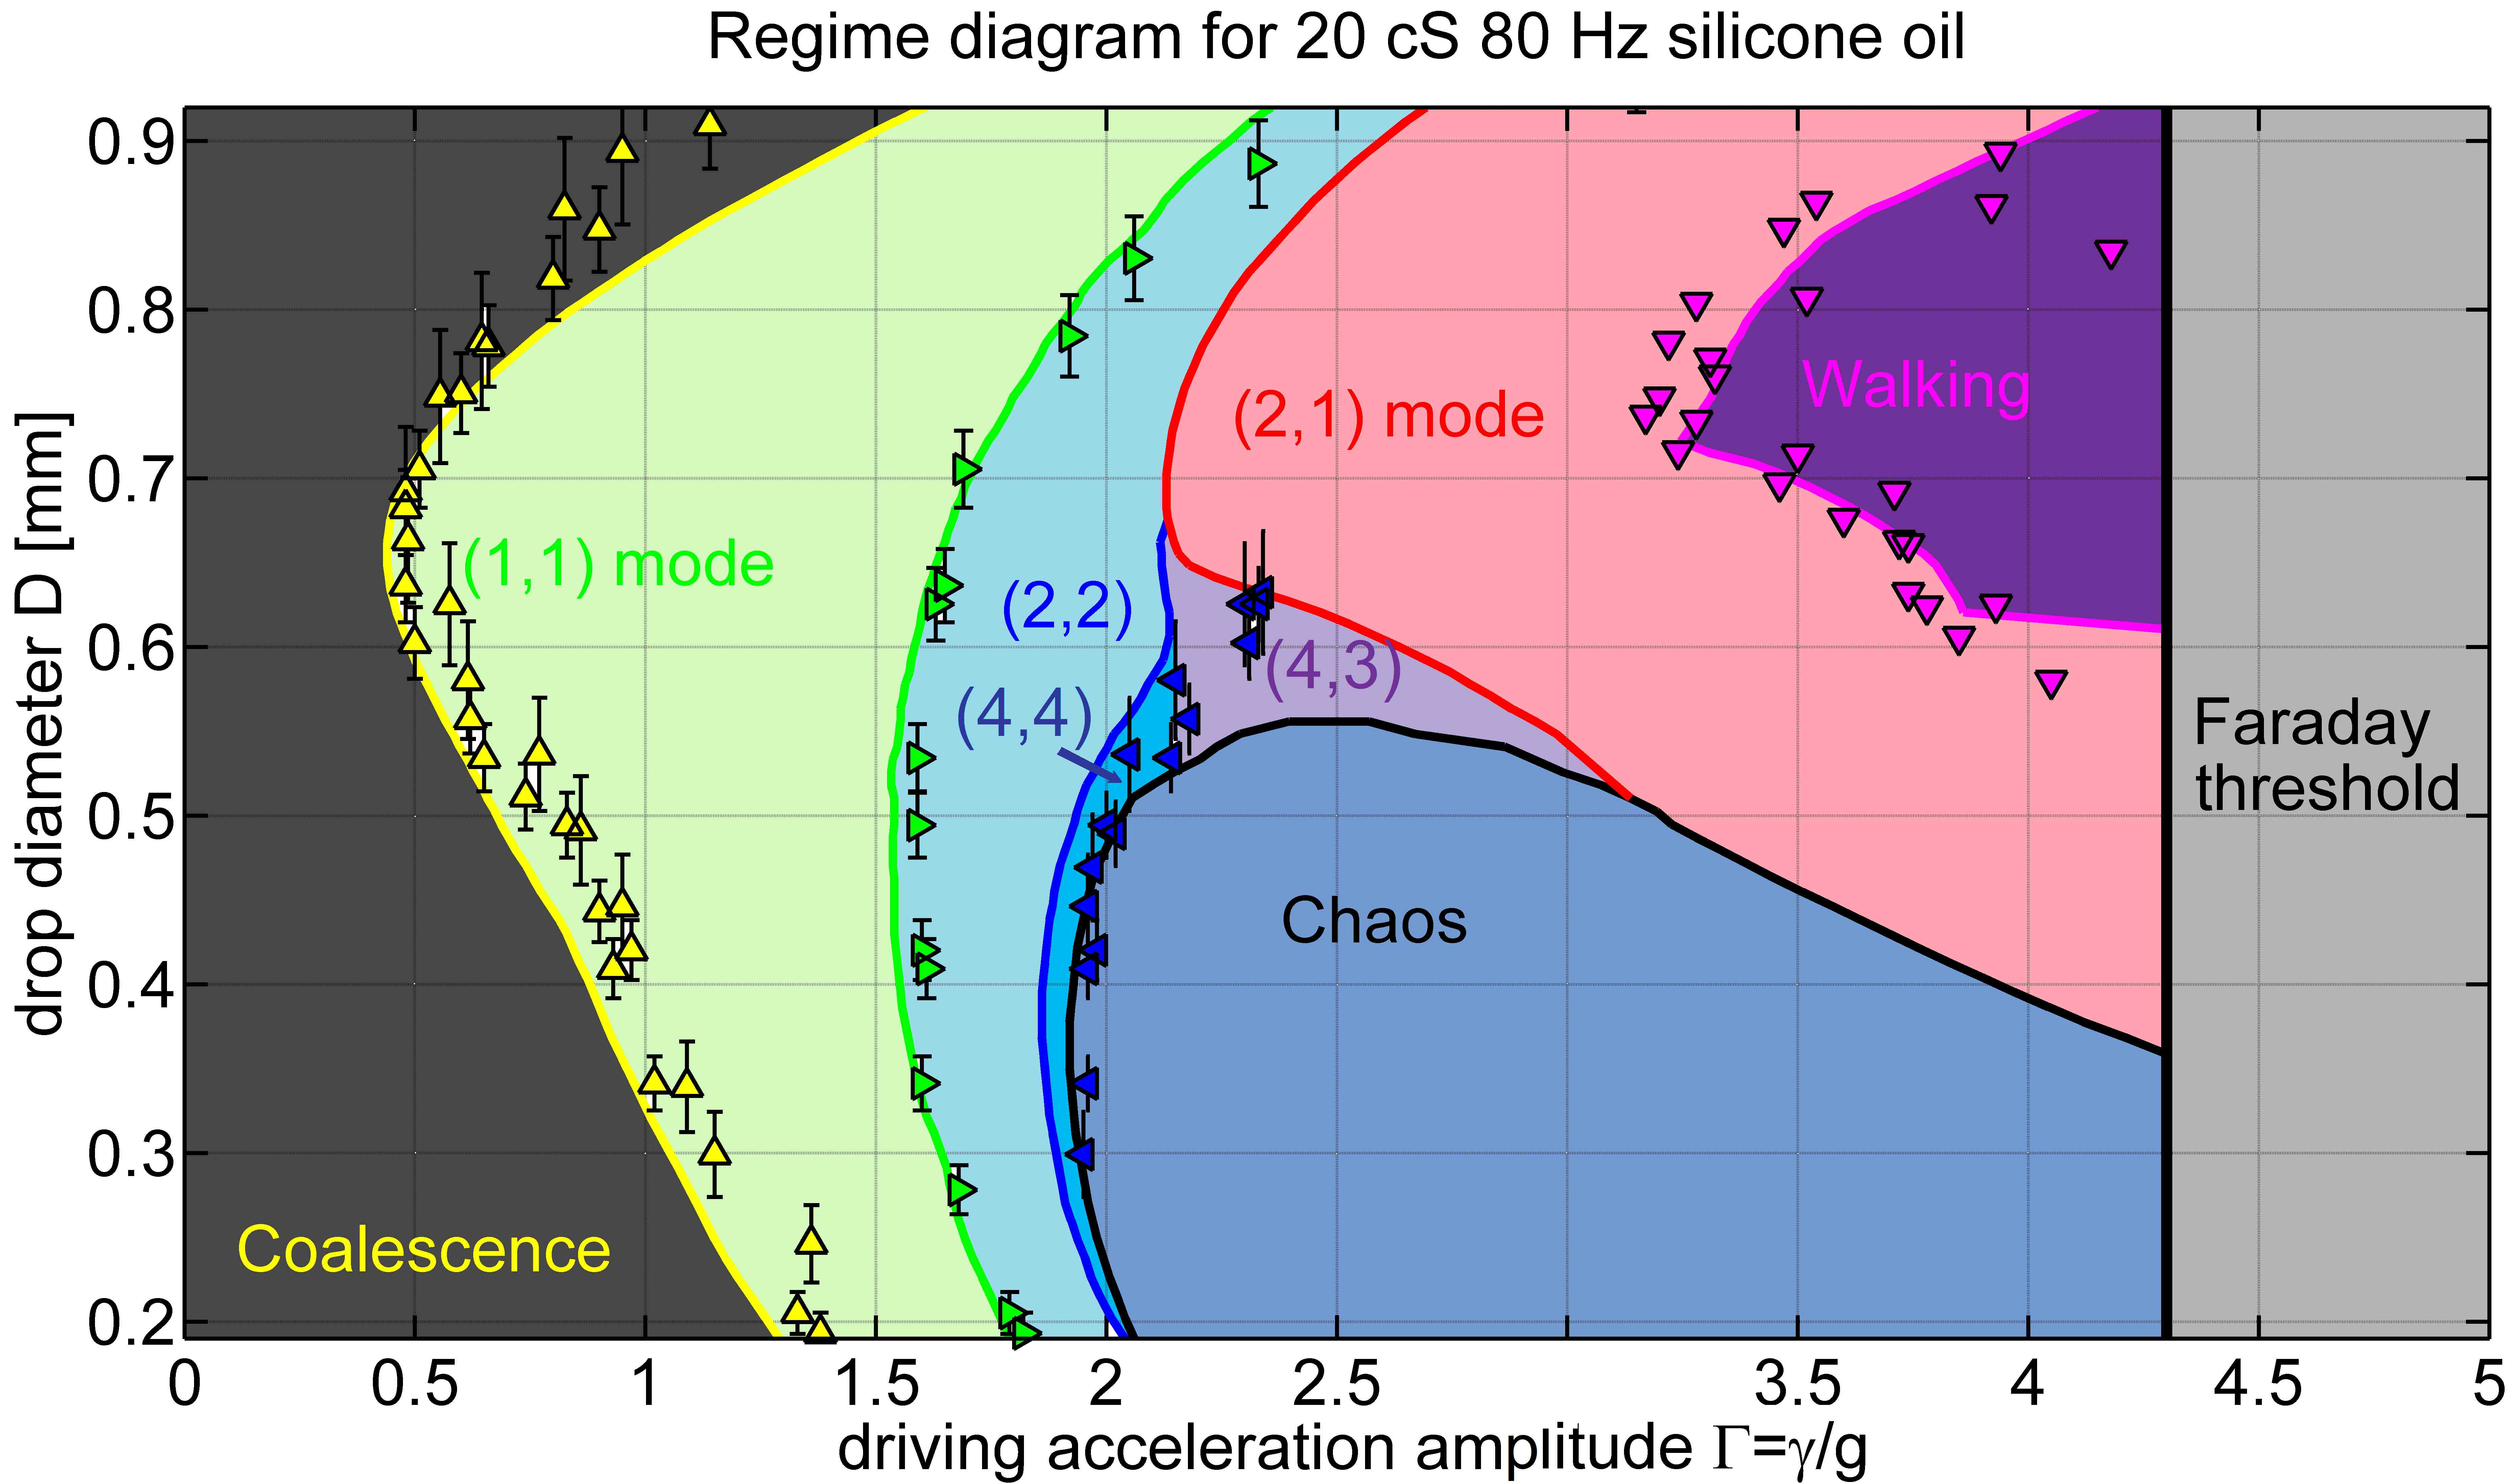
\includegraphics[scale=0.075]{Regime-Mega}
	     \caption{The different bouncing regimes for the oil drops of 20 cS silicon oil and at $f$ = $\omega / 2\pi$ = 80 Hz. The parameters ($m$,$n$) describe the droplet that bounces $n$ times in $m$ forcing periods. }
	 \label{regime}
	\end{figure}

The various modes seen in \refFig{regime} can be described by ($m$,$n$), where $n$ is the number to times the droplet contacts the surface over period $m/f$. For example, in the (1,1) mode, the droplet hits the oil bath once per driving period. In the (2,2) mode, the drop makes two bounces of differing heights. 
	       
            \subsection{Path Memory}
            Path memory is a parameter that can be varied in this setup. Every time the droplet impacts the bath, it creates a radial traveling wave. Over the course of many bounces, a wavefield composed of a superposition of the many waves arises. If the bouncing droplet impacts the wavefield in such a way that it recives a lateral force from the slope of the wave, then it will be pushed to the side slightly. The next time the droplet makes contanct with the bath, it will again be pushed to the side. This propels the bouncing droplet, causing it to walk across the surface of the bath. These ``walkers" are pushed in a direction dictated by previous impacts, and so it is said that the oil bath ``remembers" the previous bounce.	  
            
            Damping the waves results in a low-memory limit, since the walker is affected by only the previous impact. In an undamped system (approaching the Faraday threshold), the system becomes high-memory because walker can be affected by waves from many impacts ago. The quantum like features of this experiment arise in the high-memory limit. (For more, Eddi et. al, 2011b: Information stored in Faraday waves.) 

            \subsection{Single-Particle Diffraction}

	       \subsection{Tunneling}
	       The guiding wave field can be partially reflected off of an edge or even a change in depth of the oil bath. This effect can be seen when a walker is pushed back from a under-the-surface step, seemingly without any contact. In rare cases, the walker will actually tunnel across the step; that is, it will continue to walk along the surface of the oil bath and pass over the step without reflection. In the first experiment done by Eddi et al., they demonstrated tunneling by by building square "corrals" of varying thicknesses. In the second experiment, they built a rhombus shape which forced the walker across the center of a rhombus. The barrier was placed perpendicular to the direction of travel of the walker, so that it would hit the wall directly rather than at an angle (as in the square corral). ``The tunneling probability decreases exponentially with the barrier width and increases as the Faraday threshold is approached." Eddi et. al also found that the probability of tunneling increased with the velocity of the walker. (For more, Eddi et. al 2009b: Unpredictable Tunneling of a classical wave-particle association)
	       
	       
	        The unpredictability of the tunneling comes from the complex interatction between the drop and its guiding wave. 

	    \subsection{Camera Modification}
